\chapter{Preparaci\'{o}n de la miner\'{i}a de datos}

  Este cap\'{i}tulo abarca la informaci\'{o}n necesaria para entender todo el procedimiento que se llevar\'{a} a cabo para realizar las pruebas, desde la selecci\'{o}n del conjunto de datos hasta la estructura de los algoritmos para obtener los resultados. Para ello este cap\'{i}tulo se desglosa en secciones secuenciales para guiar al lector paso a paso para poder repetir el experimento.
  
  \section{Paso 1: Entendimiento, conocimientos previos e identificaci\'{o}n de la meta}

  Este es el paso inicial preparatorio donde se desarrolla el entendimiento del dominio de la aplicaci\'{o}n. Se definen las decisiones que se tomar\'{a}n en los siguientes pasos, ya sea la transformaci\'{o}n, los algoritmos, representaci\'{o}n, etc. Adem\'{a}s, se define el entorno en que se desarrollar\'{a} la aplicaci\'{o}n junto a las caracter\'{i}sticas, tecnolog\'{i}as y herramientas que se usan en el proyecto, las cuales fueron definidas en el cap\'{i}tulo anterior, por lo que en esta secci\'{o}n se procede a tomar las decisiones de los pr\'{o}ximos pasos. El objetivo que se persigue con esta metodolog\'{i}a es la predicci\'{o}n, b\'{a}sicamente en predecir satisfactoriamente la clase de los datos pasados como prueba.
  
  En la selecci\'{o}n del conjunto de datos no es necesario crear los datos ya que se utiliza un conjunto de datos extra\'{i}dos de Kaggle. Debido a ello no es necesario extraer informac'{o}n de varias fuentes e integrarlas en una estructura homog\'{e}nea.
  
  En el tercer paso se procede a realizar la limpieza de los datos en caso de ser necesario y luego se pasa al preprocesamiento. Para la limpieza es necesario detectar que los datos est\'{e}n completos y homog\'{e}neos, en caso de que existan datos incompletos en una transacci\'{o}n, se procede a ser eliminada la transacci\'{o}n del conjunto de datos. En caso de no estar homog\'{e}neos los tipos de datos por atributos y se convierten los que no pertenezcan a ese tipo. El preprocesamiento de los datos se llevar\'{a} a cabo porque existen un amplio desbalance de la informaci\'{o}n, d\'{i}gase cuando la clase minoritaria represente menos de 10\% del total de muestras del conjunto de datos, en cuyo caso se proceder\'{a} a balancear mediante los algoritmos de balanceado de informaci\'{o}n mencionados en el cap\'{i}tulo anterior. Cada uno de los conjuntos obtenidos mediante el balance de la informaci\'{o}n ser\'{a} para entrenar los modelos incluyendo la versi\'{o}n desbalanceada.

  En el cuarto paso se lleva a cabo la transformaci\'{o}n de la informaci\'{o}n, ya sea la reducci\'{o}n de dimensiones o discretizaci\'{o}n. La reducci\'{o}n de dimensiones se llevar\'{a} a cabo eliminando atributos que no sean necesarios para el preprocesamiento o extray\'{e}ndolos para que no afecten o lancen resultados ficticios. En el caso de este proyecto los datos son valores num\'{e}ricos reales, por lo tanto, no es necesario realizar la discretizaci\'{o}n.
  
  En el quinto paso se decide que m\'{e}todo de miner\'{i}a de datos usar, que es clasificaci\'{o}n debido principalmente al objetivo y a las caracter\'{i}sticas que tiene este m\'{e}todo.

  En el sexto y s\'{e}ptimo paso se eligen e implementan los algoritmos para la miner\'{i}a de datos, los cuales son de DL por el enfoque de las m\'{e}tricas de comparaci\'{o}n. Se establecer\'{a}n la estructura de cada algoritmo a emplear, adem\'{a}s de un enfoque matem\'{a}tico al funcionamiento de cada uno.

  El octavo y noveno paso, los cu\'{a}les son los \'{u}ltimos, forman parte del cap\'{i}tulo siguiente, donde se realizar\'{a}n la evaluaci\'{o}n, comparaci\'{o}n y representaci\'{o}n de los resultados de los algoritmos seleccionados. Luego de escoger los mejores algoritmos, se aplicar\'{a} el conocimiento adquirido.

\section{Paso 2: Selecci\'{o}n del conjunto de datos}

  El conjunto de datos $S$ consta de 20 000 filas con 31 columnas, es decir que, se trabaja con 20 000 transacciones de las cuales se tienen 31 caracter\'{i}sticas. De estas 31 caracter\'{i}sticas existe informaci\'{o}n privada nombradas como V1, V2, V3, hasta V28, \textit{Time} representa el instante de tiempo en que se realiz\'{o} dicha transacci\'{o}n, \textit{Amount} es la cantidad de la transacci\'{o}n realizada, y, por \'{u}ltimo, \textit{Class} tiene dos posibles valores: $0$ para las transacciones normales y $1$ para las transacciones fraudulentas.

  Del total de 20 000 muestras, 19 936 son transacciones normales y 64 son transacciones fraudulentas, representando los fraudes un 0.32\% del conjunto de muestras, evidenciando un desbalance de la informaci\'{o}n y un porcentaje inferior al 10\%. Por lo tanto, es necesario llevar a cabo un balanceado de la informaci\'{o}n en el preprocesamiento.

\begin{figure}[h!]
	\centering
	\includegraphics[width=0.5\textwidth]{"figuras/Fig4"}
	\caption{Desbalance de las clases}
\end{figure}

\section{Paso 3: Limpieza y preprocesamiento}

  La primera acci\'{o}n a realizar es verificar si los datos est\'{a}n completos y homog\'{e}neos. Luego de la verificaci\'{o}n se obtiene como resultado que los datos est\'{a}n completos y presenta su homogeneidad, como parte de este proceso de verificaci\'{o}n se presentan valores an\'{o}malos que son el prop\'{o}sito de esta investigaci\'{o}n por lo que se mantienen dentro del conjunto de datos. Una vez concluido se procede al preprocesamiento de la informaci\'{o}n.
  
  Luego de la limpieza es necesario dividir los datos en dos conjuntos, uno de entrenamiento y otro para la prueba. Debido al gran desbalance de informaci\'{o}n que poseen los datos se le aplicar\'{a}n las soluciones mencionadas en el cap\'{i}tulo anterior, aunque solo se le aplicar\'{a}n al conjunto de entrenamiento. Todos los algoritmos para solucionar el desbalance de informaci\'{o}n que se presentar\'{a}n pertenecen a la librer\'{i}a imbalanced-learn.
  
  \subsection{RandomUnderSampler}

  RandomUnderSampler aplica un algoritmo de selecci\'{o}n de prototipos que selecciona ejemplos del conjunto de datos $S$. Entonces, $S^{'}$ es definido como $|S^{'}|<|S|$ y $S^{'}\in S$. Este algoritmo es una t\'{e}cnica de submuestreo controlada, es una forma de balancear los datos seleccionando aleatoriamente un subconjunto de datos de las clases.
  
\begin{figure}[h!]
	\centering
	\includegraphics[width=0.5\textwidth]{"figuras/Fig6"}
	\caption{Aplicaci\'{o}n de UnderSampler}
\end{figure}

  UnderSampler a pesar de ser un algoritmo que soluciona el problema desbalanceado, tiene una gran desventaja y es que elimina informaci\'{o}n para el entrenamiento y el conjunto de datos se vuelve extremadamente peque\~{n}o, reduciendo la capacidad de predicci\'{o}n de los modelos.
  
  \subsection{RandomOverSampler}
  
  RandomOverSampler genera nuevos ejemplos en las clases que est\'{a}n subrepresentadas mediante el sobre muestreo aleatorio de la clase minoritaria, en otras palabras, multiplicar los datos de la clase minoritaria hasta lograr el equilibrio. Formalmente $S^{'}$ se define como $|S^{'}|>|S| y S\in S^{'}$.
  
  \begin{figure}[h!]
  	\centering
  	\includegraphics[width=0.5\textwidth]{"figuras/Fig8"}
  	\caption{Aplicaci\'{o}n de OverSampler}
  \end{figure}

  A diferencia de UnderSampler, este algoritmo no elimina informaci\'{o}n, pero no adiciona ninguna informaci\'{o}n nueva para el entrenamiento por solo repetir los datos de la clase minoritaria.
  
  \subsection{SMOTE y ADASYN}
  
    SMOTE y ADASYN generan nuevas muestras sint\'{e}ticas por interpolaci\'{o}n que difieren de las originales. La diferencia se centra en que ADASYN se enfoca en generar muestras sint\'{e}ticas junto a las muestras originales que est\'{a}n clasificadas incorrectamente usando un clasificador KNN, mientras que la implementaci\'{o}n de SMOTE no har\'{a} ninguna distinci\'{o}n entre muestras err\'{o}neas o correctas para ser clasificadas usando la regla KNN. Por lo tanto, ambos algoritmos usan el mismo algoritmo.
    
    SMOTE, a partir de una muestra $x_{i}$ de la clase minoritaria, se generar\'{a} una nueva muestra $x_{new}$ por su vecino m\'{a}s cercano $x_{zi}$, y esta nueva muestra es incluida al conjunto de datos, esto se repite hasta que los datos sean balanceados. Su ecuaci\'{o}n es:
    \begin{equation}
    	x_{new}=x_{i}+\leftthreetimes \times (x_{zi}-x_{i})
    \end{equation}
    Donde $\leftthreetimes$ es un n\'{u}mero aleatorio entre $0$ y $1$. Esta interpolaci\'{o}n crear\'{a} una muestra sobre la l\'{i}nea entre $x_{zi}$ y $x_{i}$.
    
    \begin{figure}[h!]
    	\centering
    	\includegraphics[width=0.5\textwidth]{"figuras/Fig10"}
    	\caption{Aplicaci\'{o}n de SMOTE}
    \end{figure}

    ADASYN a diferencia de SMOTE, el n\'{u}mero de muestras generadas para cada $x_{i}$ es proporcional al n\'{u}mero de muestras que no son de la misma clase que $x_{i}$ en una vecindad determinada. Por lo tanto, se generar\'{a}n m\'{a}s muestras en el \'{a}rea donde no exista una fuerte densidad de la clase minoritaria.
    
  \begin{figure}[h!]
  	\centering
  	\includegraphics[width=0.5\textwidth]{"figuras/Fig12"}
  	\caption{Aplicaci\'{o}n de ADASYN}
  \end{figure}

\subsection{Paso 4: Transformaci\'{o}n de los datos}

  Los datos poseen 31 dimensiones o atributos, la dimensi\'{a}n \textit{Class} va a ser separada del conjunto de datos y la dimensi\'{o}n \textit{Amount} ser\'{a} eliminada del preprocesamiento. Por lo tanto, se trabajar\'{a} con 29 dimensiones, mientras que la dimensi\'{o}n \textit{Class} ser\'{a} usada para clasificar los datos pre procesados y poder ser comparados con las predicciones.
  
  La divisi\'{o}n de los datos en los conjuntos de entrenamiento y prueba, se realiza con una proporci\'{o}n de 80\% para el entrenamiento y 20\% para las pruebas de forma est\'{a}ndar. No obstante, se realizar\'{a}n pruebas para comprobar cu\'{a}l es la mejor forma de dividir los grupos en cuanto a por ciento de datos para pruebas.
  
  Al entrenar los modelos es necesario realizar la estandarizaci\'{o}n y escalado de variables num\'{e}ricas. Al ser num\'{e}ricos los predictores, la escala en que se miden y la magnitud de su varianza pueden influir en gran medida en el modelo. Si no se igualan de alguna forma los predictores pueden ocasionar que las variables objetivas no dominen el modelo y la variable respuesta no guarde relaci\'{o}n con ellas. Para ello se usar\'{a} la estrategia de normalizaci\'{o}n que consiste en transformar los datos de forma que todos los predictores est\'{e}n aproximadamente en la misma escala. Sus dos variantes son:
\begin{itemize}
	\item Normalizaci\'{o}n Z-score (StandardScaler): se divide cada predictor entre su desviaci\'{o}n t\'{i}pica despu\'{e}s de haber sido centrado.
	\item Estandarizaci\'{o}n max-min (MinMaxScaler): transforma los datos de forma que est\'{e}n dentro del rango $[0,1]$.
\end{itemize}

\section{Paso 5: M\'{e}todo de miner\'{i}a de datos}

  Existen tres m\'{e}todos de miner\'{i}a de datos:
  \begin{itemize}
  	\item Regresi\'{o}n: usa algoritmos de aprendizaje supervisado para predecir y modelar variables aleatorias continuas. Es usado para cambios continuos como pron\'{o}sticos de precios de vivienda, tendencia de acciones o resultados de pruebas.
  	\item Clasificaci\'{o}n: usa algoritmos de aprendizaje supervisados para modelar o predecir variables aleatorias discretas. Se usan en varias tareas como filtrado de correo electr\'{o}nico, fraude financiero y predicci\'{o}n de cambios de empleados.
  	\item Agrupaci\'{o}n: usa algoritmos de aprendizaje no supervisado, estos encuentran los grupos \'{e}tnicos naturales de las muestras observadas bas\'{a}ndose en la estructura interna de los datos. Es usado en la segmentaci\'{o}n de clientes, agrupaci\'{o}n de noticias, recomendaci\'{o}n de art\'{i}culos, etc.
  \end{itemize}

  La predicci\'{o}n es a veces referida como una miner\'{i}a de datos supervisada, entonces el m\'{e}todo a usar es la clasificaci\'{o}n debido al enfoque del proyecto que es la detecci\'{o}n de fraude de tarjeta de cr\'{e}dito.
  
  \section{Paso 6 y 7: Elecci\'{o}n e implementaci\'{o}n de los algoritmos de miner\'{i}a de datos}
  
    A partir de la estrategia seleccionada, se selecciona en este paso los m\'{e}todos para la b\'{u}squeda de patrones. Considerando las m\'{e}tricas seleccionadas para comparar los algoritmos, se decide usar las redes neuronales, en espec\'{i}fico las pertenecientes a DL, para conocer cu\'{a}les son los algoritmos apropiados para obtener \'{o}ptimos resultados.
    
    Las redes neuronales o ANN son modelos creados al ordenar operaciones matem\'{a}ticas siguiendo determinada estructura. La forma m\'{a}s com\'{u}n de representar su estructura es mediante el uso de capas (\textit{layers}), formadas a su vez por neuronas (\textit{units} o \textit{neurons}). Cada neurona, realiza una operaci\'{o}n sencilla y est\'{a} conectada a las neuronas de la capa anterior y de la capa siguiente mediante pesos, cuya funci\'{o}n es regular la informaci\'{o}n que se propaga de una neurona a la otra.  La primera capa de la red es la capa de entrada (\textit{Input Layer}), donde se reciben los datos sin clasificar, luego pasa por la capa intermedia o capa oculta (\textit{hidden layer}) donde se reciben los datos de la capa de entrada, ponderados por los pesos. Finaliza en la \'{u}ltima capa (\textit{output layer}) donde combina los valores que salen de la capa intermedia para generar la predicci\'{o}n.
    
    La neurona es la unidad funcional de los modelos de redes, donde ocurren simplemente dos operaciones: la suma ponderada de sus entradas y la aplicaci\'{o}n de una funci\'{o}n de activaci\'{o}n. En la primera se multiplica cada valor de entrada $x_{i}$, por su peso asociado $w_{i}$ y se suman junto con la parcialidad $b$, luego este valor pasa por una funci\'{o}n, conocida como funci\'{o}n de activaci\'{o}n $a$, transformando el valor neto de entrada en un valor de salida $S$. Entonces la ecuaci\'{o}n para obtener los datos de entrada en las capas intermedias se define como $E=\sum_{i=0}^{n}x_{i}w_{i}+b_{i}$, luego la salida de la neurona se convierte en $S=a(x_{i} w_{i}+b_{i})$.
    
    Las funciones de activaci\'{o}n controlan la informaci\'{o}n que se propaga de una capa a la siguiente (\textit{forward propagation}). Entre las funciones a utilizar se encuentran las siguientes:
    
    \begin{itemize}
    	\item \textit{Rectified linear unit} (ReLU): aplica una transformaci\'{o}n no lineal donde la neurona se activa solo si la entrada est\'{a} por encima de $0$, esto hace que se retengan los valores positivos y descarta los negativos d\'{a}ndoles una activaci\'{o}n de $0$. $ReLU(x)=max(x,0)$.
    	\item Sigmoide: transforma los valores en el rango $(-\infty,+\infty)$ a valores en el rango $(0,1)$. $sigmoid(x)=\frac{1}{1+\exp(-x)}$.
    	\item Softmax: esta funci\'{o}n calcula las probabilidades relativas, parecido a sigmoid. $softmax(x)=\frac{\exp(x_{i})}{\sum_{j}\exp(z_{j})}$.
    \end{itemize}

    La funci\'{o}n de coste $l$ o funci\'{o}n de p\'{e}rdida (\textit{loss function} o \textit{cost function}), es la encargada de cuantificar la distancia entre el valor real y el predicho por la red. En el caso del m\'{e}todo de clasificaci\'{o}n, se utiliza para dirigir el entrenamiento de los modelos, por lo que se elige el m\'{e}todo \textit{binary cross-entropy loss}. Como la clasificaci\'{o}n es binaria, la variable de respuesta es $1$ o $0$, y la probabilidad $p=Pr(y=1)$. La funci\'{o}n para ello es:
    \begin{equation}
    	L_{\log} (y,Pr)=-\log Pr(y\mid p)=-(y\log(p)+(1-y)\log(1-p))
    \end{equation}
  
    El modelo de red neuronal con una \'{u}nica capa, s\'{o}lo es capaz de aprender patrones sencillos. Para romper con esta limitaci\'{o}n se combinan m\'{u}ltiples capas ocultas, permitiendo a la red aprender relaciones mucho m\'{a}s complejas entre los predictores y la variable de respuesta. Combinando m\'{u}ltiples capas ocultas y funciones de activaci\'{o}n no lineales, los modelos de redes pueden aprender pr\'{a}cticamente cualquier patr\'{o}n.
  
    En el proceso de entrenamiento de una red neuronal consiste en ajustar el valor de los pesos y parcialidad de tal forma que se obtenga el menor error posible. Debido a ello el modelo es capaz de identificar qu\'{e} predictores tiene mayor influencia y de qu\'{e} forma est\'{a}n relacionados entre ellos y con la variable respuesta. Para lograr disminuir el error se han combinado m\'{u}ltiples m\'{e}todos matem\'{a}ticos, entre ellos:
  
  \begin{itemize}
  	\item Retro propagaci\'{o}n (\textit{backpropagation}): es el algoritmo que permite cuantificar la influencia que tiene cada peso y parcialidad de la red en sus predicciones. Hace uso de la regla de la cadena para calcular el gradiente, esto permite identificar que pesos de la red hay que modificar para mejorarla.
  	\item Descenso de gradiente estoc\'{a}stico (SGD): consiste en dividir el conjunto de entrenamiento en lotes (\textit{minibatch} o \textit{batch}) y actualizar los par\'{a}metros de la red con cada uno. De esta forma en vez de esperar evaluar todas las observaciones para actualizar los par\'{a}metros, se pueden ir actualizando de forma progresiva.
  	\item Adam: es una combinaci\'{o}n de RMSprop\footnote{RMSprop: algoritmo que se utiliza para la optimizaci\'{o}n de lotes completos, intenta resolver la amplia variaci\'{o}n de las magnitudes de los gradientes.} y SGD con impulso. Utiliza los gradientes cuadrados para escalar la tasa de aprendizaje como RMSprop y aprovecha el impulso mediante el uso de la media m\'{o}vil del gradiente en lugar del gradiente como SGD con impulso \cite{33}. Es uno de los optimizadores con mayor tendencia en la actualidad.
  \end{itemize}

    Es importante mencionar que una ronda completa de iteraciones sobre todos los \textit{batchs} se llama \'{e}poca. El n\'{u}mero de \'{e}pocas con las que se entrena una red equivale al n\'{u}mero de veces que la red ve cada ejemplo de entrenamiento. Es decir que la cantidad de \'{e}pocas influye en los resultados del modelo predictor.
    
    Las redes neuronales son capaces de generar modelos que aprenden relaciones muy complejas, sin embargo, sufren f\'{a}cilmente el problema de sobreajuste (\textit{overfitting}) lo que los incapacita al tratar de predecir nuevas observaciones. La forma de minimizar este problema y conseguir modelos \'{u}tiles es configurando de forma adecuada sus hiperpar\'{a}metros:
    
    \subsubsection{N\'{u}mero y tama\~{n}o de capas}
    
    La capa de entrada tiene tantas neuronas como predictores y la capa de salida tiene tantas neuronas como clases en problemas de clasificaci\'{o}n. Cuantas m\'{a}s neuronas y capas tengan el modelo, mayor la complejidad de las relaciones que puede aprender el modelo. Sin embargo, dado que cada neurona est\'{a} conectada por pesos al resto de neuronas de las capas adyacentes, el n\'{u}mero de par\'{a}metros a aprender aumenta y con ello el tiempo de entrenamiento. Debido a ello los modelos tendr\'{a}n a lo sumo 10 capas, para lograr compensar la efectividad de los predictores con el tiempo estimado de entrenamiento.
    
    \subsubsection{Ratio de aprendizaje}
    
    La ratio de aprendizaje (\textit{learning rate}) establece c\'{o}mo de r\'{a}pido pueden cambiar los par\'{a}metros de un modelo a medida que se optimiza. Es uno de los m\'{a}s complicados de establecer, ya que depende mucho de los datos e interacciona con el resto de hiperpar\'{a}metros. Si el \textit{learning rate} es muy grande, el proceso de optimizaci\'{o}n puede ir saltando de una regi\'{o}n a otra sin que el modelo sea capaz de aprender. Por el contrario, si es muy peque\~{n}o, el proceso de entrenamiento puede demorar demasiado y no llegar a completarse.
    
    Se utiliza el \textit{learning rate} definido como est\'{a}ndar de cada optimizador, en el caso de Adam es $0.001$ y en el caso de SGD es $0.01$.
    
    \subsubsection{Algoritmo de optimizaci\'{o}n}
    
    El SGD y Adam son los algoritmos de optimizaci\'{o}n a utilizar en el proyecto, a pesar de que SGD presente problemas a medida que los modelos aumentan de tama\~{n}o. Por lo tanto, SGD es utilizado para modelos que presenten pocas neuronas y capas en el modelo, mientras que Adam ser\'{a} utilizado para conjunto de datos grandes, aunque puede ser utilizado en cualquier tipo de modelos.
    
    \subsubsection{Regularizaci\'{o}n}
    
    Los m\'{e}todos de regularizaci\'{o}n se utilizan con el objetivo de reducir el sobreajuste de los modelos. Un modelo con sobreajuste memoriza los datos de entrenamiento, pero es incapaz de predecir correctamente nuevas observaciones. Debido a que los modelos de redes neuronales pueden considerarse como modelos sobre parametrizados, se adopta el \textit{dropout} como estrategia de regularizaci\'{o}n.
    
    \textit{Dropout} consiste en desactivar aleatoriamente una serie de neuronas durante el proceso de entrenamiento. Durante cada iteraci\'{o}n del entrenamiento se ponen a cero los pesos de una fracci\'{o}n aleatoria de neuronas por capa. El porcentaje de neuronas que suele desactivarse por capa (\textit{dropout rate}) suele ser un valor entre $0.2$ y $0.5$. Por lo tanto, en el proyecto se les aplicar\'{a}n a los algoritmos tres capas de \textit{dropout} con capas intermedias, cada uno con un porcentaje de neuronas desactivadas diferentes. Para establecer el orden y porcentaje se aplicar\'{a}n experimentos con diferentes combinaciones, hasta encontrar el \'{o}ptimo.
       
    Una vez definidas las bases, opciones y estrategias a aplicar para obtener \'{o}ptimos resultados en los modelos, se procede a definir la estructura de los algoritmos seleccionados para el proyecto.
    
    \subsubsection{AutoEncoder (AE)}
    
    El AE consiste en tres partes, la capa de entrada donde se introducen los datos originales sin clasificar, la capa oculta para codificar la entrada y la capa de salida para decodificar. Usando \textit{Backpropagation}, el algoritmo se auto entrena continuamente cambiando los valores de la salida objetivo por los valores de entrada. Esto fuerza a que la capa m\'{a}s peque\~{n}a del codificador use la reducci\'{o}n dimensional para eliminar ruido y reconstruir los datos de entrada, de esta forma aprenden como comprimir los datos de la capa de entrada y luego descomprimir en cualquier formato que mejor se adecue a los datos originales. AE est\'{a} estrechamente relacionado al an\'{a}lisis de componente principal (PCA), principalmente en el cuello de botella que se encuentra en la capa m\'{a}s peque\~{n}a de la red, donde corresponde con sus principales componentes.
    
    Se puede expresar el proceso matem\'{a}ticamente, para ello se divide la red en dos partes, el codificador $\theta$ y el decodificador $\phi$, es necesario aclarar que la capa de entrada con los datos originales $X$ no se incluyen en ninguna. Adem\'{a}s, se define $F$ como la representaci\'{o}n de los datos en el cuello de botella o capa de menor dimensi\'{o}n.
    
    \begin{align}
    	\theta:X\rightarrow F \\
    	\phi:F\rightarrow X \\
    	\theta,\phi=argmin_{\theta,\phi}\| X-(\theta \thinspace o \thinspace \phi)X\|^{2}   
    \end{align}
    
    B\'{a}sicamente se intenta recrear los datos originales luego de aplicar una compresi\'{o}n no linear generalizada. En la parte codificadora puede ser representada por la funci\'{o}n de activaci\'{o}n de una red neuronal est\'{a}ndar, donde $z=\sigma(Wx+b)$ es la dimensi\'{o}n latente. De manera similar se puede representar la parte decodificadora como $x^{'}=\sigma^{'} (W^{'} z+b^{'})$.
    
    Al algoritmo AE se le aplicar\'{a} tres capas de \textit{Dropout} no consecutivas y no necesariamente con el mismo porcentaje de eliminaci\'{o}n para evitar el \textit{overfitting}; y el optimizador Adam. Posee 9 capas para su funcionamiento, que consiste en una capa de datos de entrada, cuatro capas para el codificador y cuatro capas del decodificador. Para lograr un entendimiento de la reducci\'{o}n de las dimensiones se especificar\'{a}n las dimensiones cada capa y su secuencia:
    
    \begin{enumerate}
    	\item \textit{Input Layer}: es la capa de entrada de datos, por lo tanto, se introducen los datos en bruto sin procesar, estos datos poseen 29 dimeniones.
    	\item \textit{Dense1 Layer}: Reduce las dimensiones de los datos de entrada a 14 dimensiones.
    	\item \textit{Dense2 Layer}: Reduce nuevamente las dimensiones a 7.
    	\item \textit{Dropout1 Layer}: Elimina modelos de patrones seg\'{u}n el por ciento especificado, de esta forma se evita el \textit{overfitting}.
    	\textit{Dense3 Layer}: Reduce las dimensiones a 1. Hasta este punto se realiza la codificaci\'{o}n.
    	\textit{Dropout2 Layer}: Elimina modelos de patrones nuevamente. A partir de este paso comienza la decodificaci\'{o}n.
    	\item \textit{Dense4 Layer}: Incrementa las dimensiones a 7 de forma tal que va clasificando los datos.
    	\item \textit{Dropout3 Layer}: Elimina patrones nuevamente.
    	\item \textit{Dense5 Layer}: Incrementa las dimensiones a 29, igual que las dimensiones de entrada.
    	\item \textit{Dense6 Layer} o \textit{Output Layer}: Comprime las dimensiones a 1 y concluye la clasificaci\'{o}n.
    \end{enumerate}

\begin{figure}[h!]
	\centering
	\begin{tikzpicture}[shorten >=1pt,->,draw=black!50, node distance=\layersep]
		\tikzstyle{every pin edge}=[<-,shorten <=1pt]
		\tikzstyle{neuron}=[circle,fill=black!25,minimum size=17pt,inner sep=0pt]
		\tikzstyle{input neuron}=[neuron, fill=green!50];
		\tikzstyle{decoder neuron}=[neuron, fill=red!50];
		\tikzstyle{encoder neuron}=[neuron, fill=blue!50];
		\tikzstyle{annot} = [text width=4em, text centered]
		
		% Draw the input layer nodes
		\foreach \y in {1,...,7}{
			% This is the same as writing \foreach \name / \y in {1/1,2/2,3/3,4/4}
			\ifnum\y<4
			\node[input neuron, pin=left: \y] (I-\y) at (0,-\y) {};
			\fi
			\ifnum\y=4
			\node[input neuron, pin=left: \vdots] (I-\y) at (0,-\y) {};
			\fi
			\ifnum\y=5
			\node[input neuron, pin=left: 27] (I-\y) at (0,-\y) {};
			\fi
			\ifnum\y=6
			\node[input neuron, pin=left: 28] (I-\y) at (0,-\y) {};
			\fi
			\ifnum\y=7
			\node[input neuron, pin=left: 29] (I-\y) at (0,-\y) {};
			\fi
		}
		
		% Draw the Dense_1 layer nodes
		\foreach \y in {2,3,4,5,6}{
			\node[encoder neuron, right of=I-4] (H1-\y) at (\layersep,-\y cm) {};
		}
		% Draw the Dense_2 layer nodes
		\foreach \y in {3,4,5}{
			\node[encoder neuron, right of=H1-3] (H2-\y) at (\layersep*2.5,-\y cm) {};
		}
		% Draw the Dropout_1 layer nodes
		\foreach \y in {3,4,5}{
			\node[encoder neuron, right of=H2-2] (H3-\y) at (\layersep*4.3,-\y cm) {};
		}
		% Draw the Dense_3 layer nodes
		\foreach \y in {4}
		\node[encoder neuron, right of=H3-2] (H4-\y) at (\layersep*5.5,-\y cm) {};
		
		% Draw the Dropout_2 layer nodes
		\foreach \y in {4}
		\node[decoder neuron, right of=H4-1] (H5-\y) at (\layersep*7,-\y cm) {};
		
		% Draw the Dense_4 layer nodes
		\foreach \y in {3,4,5}
		\node[decoder neuron, right of=H5-1] (H6-\y) at (\layersep*8.5,-\y cm) {};
		
		% Draw the Dropout_3 layer nodes
		\foreach \y in {3,4,5}
		\node[decoder neuron, right of=H6-2] (H7-\y) at (\layersep*10,-\y cm) {};
		
		% Draw the output layer node
		\foreach \y in {1,...,7}
		\node[decoder neuron, right of=H7-2] (H8-\y) at (\layersep*11.5,-\y cm){};
		
		% Connect every node in the input layer with every node in the
		% Dense_1 layer.
		\foreach \source in {1,...,7}
		\foreach \dest in {2,3,4,5,6}
		\path (I-\source) edge (H1-\dest);
		% Connect every node in the Dense_1 layer with every node in the
		% Dense_2 layer.
		\foreach \source in {2,3,4,5,6}
		\foreach \dest in {3,4,5}
		\path (H1-\source) edge (H2-\dest);
		% Connect every node in the Dense_2 layer with every node in the
		% Dropout_1 layer.
		\foreach \source in {3,4,5}
		\foreach \dest in {3,4,5}
		\path (H2-\source) edge (H3-\dest);
		% Connect every node in the Dropout_1 layer with every node in the
		% Dense_3 layer.
		\foreach \source in {3,4,5}
		\path (H3-\source) edge (H4-4);
		% Connect every node in the Dense_3 layer with every node in the
		% Dropout_2 layer.
		\path (H4-4) edge (H5-4);
		% Connect every node in the Dropout_2 layer with every node in the
		% Dense_4 layer.
		\foreach \dest in {3,4,5}
		\path (H5-4) edge (H6-\dest);
		% Connect every node in the Dense_4 layer with every node in the
		% Dropout_3 layer.
		\foreach \source in {3,4,5}
		\foreach \dest in {3,4,5}
		\path (H6-\source) edge (H7-\dest);
		% Connect every node in the Dropout_3 layer with every node in the
		% Dense_5 layer.
		\foreach \source in {3,4,5}
		\foreach \dest in {1,...,7}
		\path (H7-\source) edge (H8-\dest);
		
		% Annotate the layers
		\node[annot,above of=H1-2, node distance=1cm] {Dense1 layer};
		\node[annot,above of=H2-3, node distance=1cm] {Dense2 layer};
		\node[annot,above of=H3-3, node distance=1cm] {Dropout1 layer};
		\node[annot,above of=H4-4, node distance=1cm] {Dense3 layer};
		\node[annot,above of=H5-4, node distance=1cm] {Dropout2 layer};
		\node[annot,above of=H6-3, node distance=1cm] {Dense4 layer};
		\node[annot,above of=H7-3, node distance=1cm] {Dropout3 layer};
		\node[annot,above of=I-1] {Input layer};
		\node[annot,above of=H8-1] {Output layer};
	\end{tikzpicture}
\caption{Modelo AE}
\end{figure}

\subsubsection{Denoising AutoEncoder (DAE)}

  DAE es una versi\'{o}n estoc\'{a}stica de AE que reduce el riesgo del aprendizaje de la funci\'{o}n identidad. En AE si existen m\'{a}s capas ocultas que entradas, existe el riesgo de que el algoritmo solo aprenda la funci\'{o}n identidad durante el entrenamiento, es cuando la salida es igual a la entrada, entonces se hace inservible el algoritmo. DAE corrompe aleatoriamente los datos de entrada para reducir este riesgo y aprenda a reconstruir los datos originales a partir de los datos corruptos.
  
  Para la corrupci\'{o}n de los datos se aplicar\'{a} un m\'{e}todo que aplica ruido gaussiano aditivo centrado en cero, esto ayuda a mitigar el \textit{overfitting} y es una opci\'{o}n com\'{u}n para el proceso de corrupci\'{o}n para valores reales de entrada. No se aplicar\'{a} el \textit{dropout} y se utilizar\'{a} el optimizador SGD. En cuanto a las capas se comporta similar al AE: posee la capa de entrada de datos, cuatro capas para el codificador y dos capas para el decodificador. Secuencialmente se conforman de la siguiente forma:

\begin{enumerate}
	\item \textit{Input Layer}: La capa de entrada donde se introducen en la red los datos originales.
	\item \textit{Gaussian Noise}: En esta capa se corrompen los datos y comienza el proceso de codificaci\'{o}n.
	\item \textit{Dense1 Layer}: Se reducen las dimensiones a 14.
	\item \textit{Dense2 Layer}: Se reducen las dimensiones a 7.
	\item \textit{Dense3 Layer}: Se reducen las dimensiones a 1. Termina el proceso de codificaci\'{o}n
	\item \textit{Dense4 Layer}: Se incrementan las dimensiones 7. Comienza la decodificaci\'{o}n.
	\item \textit{Dense5 Layer}: Se incrementan las dimensiones a 29.
	\item \textit{Dense6 Layer} o \textit{Output Layer}: Se comprimen los datos a una dimensi\'{o}n. Termina la decodificaci\'{o}n.
\end{enumerate}

\begin{figure}[h!]
	\centering
	\begin{tikzpicture}[shorten >=1pt,->,draw=black!50, node distance=\layersep]
		\tikzstyle{every pin edge}=[<-,shorten <=1pt]
		\tikzstyle{neuron}=[circle,fill=black!25,minimum size=17pt,inner sep=0pt]
		\tikzstyle{input neuron}=[neuron, fill=green!50];
		\tikzstyle{decoder neuron}=[neuron, fill=red!50];
		\tikzstyle{encoder neuron}=[neuron, fill=blue!50];
		\tikzstyle{annot} = [text width=4em, text centered]
		
		% Draw the input layer nodes
		\foreach \y in {1,...,7}{
			% This is the same as writing \foreach \name / \y in {1/1,2/2,3/3,4/4}
			\ifnum\y<4
			\node[input neuron, pin=left: \y] (I-\y) at (0,-\y) {};
			\fi
			\ifnum\y=4
			\node[input neuron, pin=left: \vdots] (I-\y) at (0,-\y) {};
			\fi
			\ifnum\y=5
			\node[input neuron, pin=left: 27] (I-\y) at (0,-\y) {};
			\fi
			\ifnum\y=6
			\node[input neuron, pin=left: 28] (I-\y) at (0,-\y) {};
			\fi
			\ifnum\y=7
			\node[input neuron, pin=left: 29] (I-\y) at (0,-\y) {};
			\fi
		}
		
		% Draw the Gaussian_Noise nodes
		\foreach \y in {1,...,7}
		\node[encoder neuron] (H1-\y) at (\layersep*2,-\y) {};
		
		% Draw the Dense_1 layer nodes
		\foreach \y in {2,3,4,5,6}{
			\node[encoder neuron, right of=1-4] (H2-\y) at (\layersep*3,-\y cm) {};
		}
		% Draw the Dense_2 layer nodes
		\foreach \y in {3,4,5}{
			\node[encoder neuron, right of=H2-4] (H3-\y) at (\layersep*4.8,-\y cm) {};
		}
		% Draw the Dense_3 layer nodes
		\foreach \y in {4}
		\node[encoder neuron, right of=H3-4] (H4-\y) at (\layersep*6,-\y cm) {};
		
		% Draw the Dense_4 layer nodes
		\foreach \y in {3,4,5}
		\node[decoder neuron, right of=H4-4] (H5-\y) at (\layersep*7,-\y cm) {};
		
		% Draw the Dense_5 layer node
		\foreach \y in {1,...,7}
		\node[decoder neuron, right of=H5-4] (H6-\y) at (\layersep*9,-\y cm){};
		
		% Draw the Dense_6 layer node
		\node[decoder neuron, right of=H6-4] (O-4) at (\layersep*11,-4 cm){};
		
		% Connect every node in the input layer with every node in the
		% Gaussian_Noise layer.
		\foreach \source in {1,...,7}
		\foreach \dest in {1,...,7}
		\path (I-\source) edge (H1-\dest);
		% Connect every node in the Gaussian_Noise layer with every node in the
		% Dense_1 layer.
		\foreach \source in {1,...,7}
		\foreach \dest in {2,3,4,5,6}
		\path (H1-\source) edge (H2-\dest);
		% Connect every node in the Dense_1 layer with every node in the
		% Dense_2 layer.
		\foreach \source in {2,3,4,5,6}
		\foreach \dest in {3,4,5}
		\path (H2-\source) edge (H3-\dest);
		% Connect every node in the Dense_2 layer with every node in the
		% Dense_3 layer.
		\foreach \source in {3,4,5}
		\path (H3-\source) edge (H4-4);
		% Connect every node in the Denes_3 layer with every node in the
		% Dense_4 layer.
		\foreach \dest in {3,4,5}
		\path (H4-4) edge (H5-\dest);
		% Connect every node in the Dense_4 layer with every node in the
		% Dense_5 layer.
		\foreach \source in {3,4,5}
		\foreach \dest in {1,...,7}
		\path (H5-\source) edge (H6-\dest);
		
		% Connect every node in the Dense_5 layer with every node in the
		% Dense_6 layer.
		\foreach \source in {1,...,7}
		\path (H6-\source) edge (O-4);
		
		% Annotate the layers
		\node[annot,above of=H1-1, node distance=1cm] {Gaussian Noise layer};
		\node[annot,above of=H2-2, node distance=1cm] {Dense1 layer};
		\node[annot,above of=H3-3, node distance=1cm] {Dense2 layer};
		\node[annot,above of=H4-4, node distance=1cm] {Dense3 layer};
		\node[annot,above of=H5-3, node distance=1cm] {Dense4 layer};
		\node[annot,above of=H6-1, node distance=1cm] {Dense5 layer};
		\node[annot,above of=I-1] {Input layer};
		\node[annot,above of=O-4] {Output layer};
	\end{tikzpicture}
\caption{Modelo DAE}
\end{figure}

\subsubsection{Convolutional Neural Network (CNN)}

  La CNN es una red multicapa que consta de capas convolucionales y de reducci\'{o}n alternada, y al final tiene capas de conexi\'{o}n total como una red perceptr\'{o}n multicapa. Son capaces de detectar caracter\'{i}sticas simples y componer en caracter\'{i}sticas m\'{a}s complejas hasta detectar lo que se busca. Su principal ventaja es que cada parte de la red se le entrena para realizar una tarea, esto reduce significativamente el n\'{u}mero de capas ocultas, por lo que el entrenamiento es m\'{a}s r\'{a}pido.
  
  Al aplicar CNN para la clasificaci\'{o}n se realiza en dos fases: la primera fase es la de extracci\'{o}n de caracter\'{i}sticas, la cual est\'{a} compuesta por neuronas convolucionales y de reducci\'{o}n de muestreo; y la segunda fase es la clasificaci\'{o}n final a partir de las caracter\'{i}sticas extra\'{i}das.
  
  La primera fase se compone de capas alternas de neuronas convolucionales y neuronas de reducci\'{o}n de muestreo. A medida que los datos avanzan por esta fase, van perdiendo dimensionalidad, siendo las neuronas de las capas finales poco sensibles a perturbaciones en los datos de entrada, al mismo tiempo se activan por caracter\'{i}sticas m\'{a}s complejas. Las neuronas son remplazadas por procesadores en matriz que realizan una operaci\'{o}n sobre los datos que pasan por ellas en vez de un \'{u}nico valor num\'{e}rico. Matem\'{a}ticamente la salida $S_{j}$ de una neurona $j$, es una matriz que se calcula por medio de la combinaci\'{o}n lineal de las salidas $S_{i}$ de las neuronas de la capa anterior, cada una de ellas operadas con el n\'{u}cleo de convolucional $K_{ij}$ correspondiente a esa conexi\'{o}n. Esta cantidad es sumada a una parcialidad $b_{j}$ y luego se pasa por una funci\'{o}n de activaci\'{o}n $g$. Pr\'{a}cticamente la ecuaci\'{o}n queda de la siguiente manera:

\begin{equation}
	S_{j}=g(b_{j}+\sum_{i}(K_{ij}\otimes Y_{i})
\end{equation}

  Las CNN anteriormente utilizaban el proceso de submuestreo para realizar la reducci\'{o}n de muestreo, pero con estudios recientes se han encontrado otras operaciones como \textit{max-pooling}, que encuentra el valor m\'{a}ximo entre una ventana de muestra y pasa este valor como resumen de caracter\'{i}sticas sobre esta \'{a}rea. Esto permite que el tama\~{n}o de los datos se reduce por un factor igual al tama\~{n}o de la ventana de muestra sobre la cual se opera.
  
  Al concluir con las extracciones de caracter\'{i}sticas, se procede a la fase de clasificaci\'{o}n, gracias a que los datos han sido depurados hasta una serie de caracter\'{i}sticas \'{u}nicas para los datos de entrada. Las neuronas en esta fase funcionan de manera similar a las de un perceptr\'{o}n multicapa. La salida $y_{j}$ de una neurona $j$ se calcula a partir de las salidas $y_{i}$ de las neuronas de la capa anterior cada una de ellas multiplicadas con el peso $w_{ij}$ correspondiente. Esta cantidad es sumada a una parcialidad $b_{j}$ y luego se pasa por una funci\'{o}n de activaci\'{o}n $g$. La ecuaci\'{o}n queda de esta forma:

\begin{equation}
	y_{i}=g(b_{j}+\sum_{i}w_{ij}y_{i})
\end{equation}

  Para el proyecto se desarrollar\'{a} una CNN con dos fases de extracci\'{o}n de caracter\'{i}sticas, en cada una se aplicar\'{a} la convoluci\'{o}n, un \textit{BatchNormalization} y un \textit{Dropout}. Luego una fase de clasificaci\'{o}n donde se aplicar\'{a} un \textit{Flatten} para reducir los datos a una dimensi\'{o}n, una capa \textit{Dense} para incrementar las dimensiones a 64 y por \'{u}ltimo un \textit{Dropout}. Y, por \'{u}ltimo, una capa de salida; adem\'{a}s se aplicar\'{a} Adam como optimizador. Las capas en orden se describen a continuaci\'{o}n:
  
  \begin{enumerate}
  	\item \textit{Input Layer}: Se introducen los datos con dimensi\'{o}n $(None, 29, 1)$.
  	\item \textit{Conv1D-1 Layer}: Comienza la primera fase de extracci\'{o}n de caracter\'{i}sticas, introduciendo una capa convolucional que transforma las dimensiones a $(None, 28, 32)$.
  	\item \textit{Batch-Normalization-1 Layer}: Se aplica el regularizador para normalizar los datos.
  	\item \textit{Dropout-1 Layer}: Se aplica el regularizador para eliminar modelos para evitar el \textit{overfitting}, y culmina la primera fase de extracci\'{o}n de caracter\'{i}sticas.
  	\item \textit{Conv1D-2 Layer}: Se aplica una capa de convoluci\'{o}n y comienza la segunda fase de extracci\'{o}n de caracter\'{i}sticas. La dimensi\'{o}n de los datos se transforma a $(None, 27, 64)$.
  	\item \textit{Batch-Normalization-2 Layer}: Se aplica el regularizador para normalizar los datos.
  	\item \textit{Dropout-2 Layer}: Se aplica el regularizador para eliminar modelos para evitar el \textit{overfitting} y termina la segunda fase de extracci\'{o}n.
  	\item \textit{Flatten Layer}: Se descomponen los datos a tener la dimensi\'{o}n $(None, 1728)$ y comienza la fase de clasificaci\'{o}n.
  	\item \textit{Dense-1 Layer}: Se comprimen los datos hasta obtener las dimensiones $(None, 64)$.
  	\item \textit{Dropout-3 Layer}: Se eliminan modelos para evitar el \textit{overfitting}.
  	\item \textit{Dense-2 Layer} o \textit{Output Layer}: Se comprimen los datos una dimensi\'{o}n obteniendo los datos clasificados y terminando la fase de clasificaci\'{o}n.
  \end{enumerate}

\begin{figure}[h!]
	\centering
	\begin{tikzpicture}[shorten >=1pt,->,draw=black!50, node distance=\layersep]
		\tikzstyle{every pin edge}=[<-,shorten <=1pt]
		\tikzstyle{neuron}=[circle,fill=black!25,minimum size=17pt,inner sep=0pt]
		\tikzstyle{input neuron}=[neuron, fill=green!50];
		\tikzstyle{fase1 neuron}=[neuron, fill=blue!50];
		\tikzstyle{fase2 neuron}=[neuron, fill=green!50];
		\tikzstyle{fase3 neuron}=[neuron, fill=orange!50];
		\tikzstyle{output neuron}=[neuron, fill=red!50];
		\tikzstyle{annot} = [text width=4em, text centered]
		
		% Draw the input layer nodes
		\foreach \y in {1,...,7}{
			% This is the same as writing \foreach \name / \y in {1/1,2/2,3/3,4/4}
			\ifnum\y<4
			\node[input neuron, pin=left: \y] (I-\y) at (0,-\y) {};
			\fi
			\ifnum\y=4
			\node[input neuron, pin=left: \vdots] (I-\y) at (0,-\y) {};
			\fi
			\ifnum\y=5
			\node[input neuron, pin=left: 27] (I-\y) at (0,-\y) {};
			\fi
			\ifnum\y=6
			\node[input neuron, pin=left: 28] (I-\y) at (0,-\y) {};
			\fi
			\ifnum\y=7
			\node[input neuron, pin=left: 29] (I-\y) at (0,-\y) {};
			\fi
		}
		
		% Draw the Conv1D_1 nodes
		\foreach \y in {1,...,6}
		\node[fase1 neuron, right of=I-4] (H1-\y) at (\layersep*0.5,-\y) {};
		
		% Draw the Batch_Normalization_1 nodes
		\foreach \y in {1,...,6}
		\node[fase1 neuron, right of=H1-4] (H2-\y) at (\layersep*2.1,-\y) {};
		
		% Draw the Dropout_1 layer nodes
		\foreach \y in {1,...,6}
		\node[fase1 neuron, right of=H2-4] (H3-\y) at (\layersep*3.6,-\y cm) {};
		
		% Draw the Conv1D_2 nodes
		\foreach \y in {1,...,5}
		\node[fase2 neuron, right of=H3-4] (H4-\y) at (\layersep*5.4,-\y cm) {};
		
		% Draw the Batch_Normalization_2 nodes
		\foreach \y in {1,...,5}
		\node[fase2 neuron, right of=H4-4] (H5-\y) at (\layersep*7.1,-\y) {};
		
		% Draw the Dropout_2 layer nodes
		\foreach \y in {1,...,5}
		\node[fase2 neuron, right of=H5-4] (H6-\y) at (\layersep*8.6,-\y cm) {};
		
		% Draw the Flatten layer nodes
		\node[fase3 neuron, right of=H6-4] (H7-1) at (\layersep*10.3,-1 cm) {};
		
		% Draw the Dense_1 layer nodes
		\node[fase3 neuron, right of=H7-1] (H8-1) at (\layersep*11.7,-1 cm) {};
		
		% Draw the Dropout_3 layer nodes
		\node[fase3 neuron, right of=H8-1] (H9-1) at (\layersep*13.2,-1 cm) {};
		
		% Draw the Dense_2 layer nodes
		\node[output neuron, right of=H9-1] (H10-1) at (\layersep*15,-1 cm) {};
		
		% Connect every node in the input layer with every node in the
		% Conv1D_2 layer.
		\foreach \source in {1,...,7}
		\foreach \dest in {1,...,6}
		\path (I-\source) edge (H1-\dest);
		% Connect every node in the Conv1D_2 layer with every node in the
		% Batch_Normalization_1 layer.
		\foreach \source in {1,...,6}
		\foreach \dest in {1,...,6}
		\path (H1-\source) edge (H2-\dest);
		% Connect every node in the Batch_Normalization_1 layer with every node in the
		% Dropout_1 layer.
		\foreach \source in {1,...,6}
		\foreach \dest in {1,...,6}
		\path (H2-\source) edge (H3-\dest);
		% Connect every node in the Dropout_1 layer with every node in the
		% Conv1D_2 layer.
		\foreach \source in {1,...,6}
		\foreach \dest in {1,...,5}
		\path (H3-\source) edge (H4-\dest);
		% Connect every node in the Conv1D_2 layer with every node in the
		% Batch_Normalization_1 layer.
		\foreach \source in {1,...,5}
		\foreach \dest in {1,...,5}
		\path (H4-\source) edge (H5-\dest);
		% Connect every node in the Batch_Normalization_1 layer with every node in the
		% Dropout_2 layer.
		\foreach \source in {1,...,5}
		\foreach \dest in {1,...,5}
		\path (H5-\source) edge (H6-\dest);
		% Connect every node in the Dropout_2 layer with every node in the
		% Flatten layer.
		\foreach \source in {1,...,5}
		\path (H6-\source) edge (H7-1);
		% Connect every node in the Flatten layer with every node in the
		% Dense_1 layer.
		\path (H7-1) edge (H8-1);
		% Connect every node in the Dense_1 layer with every node in the
		% Dropout_3 layer.
		\path (H8-1) edge (H9-1);
		% Connect every node in the Dropout_3 layer with every node in the
		% Dense_2 layer.
		\path (H9-1) edge (H10-1);
		
		% Annotate the layers
		\node[annot,above of=H1-1, node distance=1cm] {Conv1D1 layer};
		\node[annot,above of=H2-1, node distance=1cm] {Batch Normalization1};
		\node[annot,above of=H3-1, node distance=1cm] {Dropout1 layer};
		\node[annot,above of=H4-1, node distance=1cm] {Conv1D2 layer};
		\node[annot,above of=H5-1, node distance=1cm] {Batch Normalization2};
		\node[annot,above of=H6-1, node distance=1cm] {Dropout2 layer};
		\node[annot,above of=H7-1, node distance=1cm] {Flatten layer};
		\node[annot,above of=H8-1, node distance=1cm] {Dense1 layer};
		\node[annot,above of=H9-1, node distance=1cm] {Dropout3 layer};
		\node[annot,above of=I-1] {Input layer};
		\node[annot,above of=H10-1] {Output layer};
	\end{tikzpicture}
	\caption{Modelo CNN}
\end{figure}

\subsubsection{Backpropagation Neural Network (BPNN)}

  En las redes neuronales se introducen los datos por la capa de entrada y se propagan hacia adelante atravesando las capas ocultas hasta llegar a la capa de salida, obteniendo el resultado final. Este resultado se compara con los valores reales para calcular el error que se comete, y propagar este error hacia atr\'{a}s a trav\'{e}s de la red neuronal, permitiendo ajustar los pesos durante el proceso de entrenamiento. Uno de los m\'{e}todos para realizar esta operaci\'{o}n es \textit{backpropagation}.
  
  \textit{Backpropagation} se activa luego de que la informaci\'{o}n llega a la capa de salida y se mide el error que se ha cometido en esa observaci\'{o}n. En la propagaci\'{o}n hacia atr\'{a}s, se van actualizando los pesos de cada conexi\'{o}n neuronal, dependiendo de la responsabilidad del peso actualizado en el error cometido. Este proceso se repite para el conjunto de observaciones, al pasar todas las observaciones por la red neuronal, se completa una \'{e}poca.
  
  Matem\'{a}ticamente el nodo de una red neuronal se podr\'{i}a representar como $a_{i}^{k}$ donde $i$ es el lugar que representa el nodo dentro de una capa y $k$ representa la capa en que se encuentra el nodo. El peso de las conexiones se representa como $w_{ji}^{k}$ donde $i$ indica el n\'{u}mero de la neurona dentro de la capa final de la conexi\'{o}n, e $j$ indica el n\'{u}mero de la neurona de la capa inicial de la conexi\'{o}n. Entonces la ecuaci\'{o}n para calcular \textit{backpropagation} queda de la siguiente forma:

\begin{align}
	a_{i}^{k}=f(u_{i}^{k}+\sum_{j=1}^{n_{k}-1}a_{j}^{k-1}w_{ji}^{k-1}) \\
	i = 1, ...., n_{k}
\end{align}

  El algoritmo BPNN que se utilizar\'{a} en el proyecto hace uso del optimizador Adam y posee solamente $5$ capas, incluyendo la de entrada y salida. A continuaci\'{o}n, la secuencia de las capas:
  
  \begin{enumerate}
  	\item \textit{Input layer}: se introducen el conjunto de datos originales sin clasificar.
  	\item \textit{Dense-1 layer}: se comprimen los datos a 14 dimensiones.
  	\item \textit{Dense-2 layer}: se comprimen los datos a 2 dimensiones.
  	\item \textit{Dense-3 layer}: se descomprimen los datos a 14 dimensiones.
  	\item \textit{Dense-4 layer} o \textit{Output layer}: se comprimen los datos a una dimensi\'{o}n y termina la clasificaci\'{o}n de los datos.
  \end{enumerate}

\begin{figure}[h!]
	\centering
	\begin{tikzpicture}[shorten >=1pt,->,draw=black!50, node distance=\layersep]
		\tikzstyle{every pin edge}=[<-,shorten <=1pt]
		\tikzstyle{neuron}=[circle,fill=black!25,minimum size=17pt,inner sep=0pt]
		\tikzstyle{input neuron}=[neuron, fill=green!50];
		\tikzstyle{hidden neuron}=[neuron, fill=blue!50];
		\tikzstyle{output neuron}=[neuron, fill=red!50];
		\tikzstyle{annot} = [text width=4em, text centered]
		
		% Draw the input layer nodes
		\foreach \y in {1,...,7}{
			% This is the same as writing \foreach \name / \y in {1/1,2/2,3/3,4/4}
			\ifnum\y<4
			\node[input neuron, pin=left: \y] (I-\y) at (0,-\y) {};
			\fi
			\ifnum\y=4
			\node[input neuron, pin=left: \vdots] (I-\y) at (0,-\y) {};
			\fi
			\ifnum\y=5
			\node[input neuron, pin=left: 27] (I-\y) at (0,-\y) {};
			\fi
			\ifnum\y=6
			\node[input neuron, pin=left: 28] (I-\y) at (0,-\y) {};
			\fi
			\ifnum\y=7
			\node[input neuron, pin=left: 29] (I-\y) at (0,-\y) {};
			\fi
		}
		
		% Draw the Dense_1 nodes
		\foreach \y in {1,...,5}
		\node[hidden neuron, right of=I-4] (H1-\y) at (\layersep*0.5,-\y) {};
		
		% Draw the Dense_2 nodes
		\foreach \y in {1,2}
		\node[hidden neuron, right of=H1-3] (H2-\y) at (\layersep*2.3,-\y) {};
		
		% Draw the Dense_3 layer nodes
		\foreach \y in {1,...,5}
		\node[hidden neuron, right of=H2-2] (H3-\y) at (\layersep*3.8,-\y cm) {};
		
		% Draw the Dense_4 nodes
		\node[output neuron, right of=H3-3] (O-1) at (\layersep*5.6,-1 cm) {};
		
		% Connect every node in the input layer with every node in the
		% Dense_1 layer.
		\foreach \source in {1,...,7}
		\foreach \dest in {1,...,5}
		\path (I-\source) edge (H1-\dest);
		% Connect every node in the Dense_1 layer with every node in the
		% Dense_2 layer.
		\foreach \source in {1,...,5}
		\foreach \dest in {1,2}
		\path (H1-\source) edge (H2-\dest);
		% Connect every node in the Dense_2 layer with every node in the
		% Dense_3 layer.
		\foreach \source in {1,2}
		\foreach \dest in {1,...,5}
		\path (H2-\source) edge (H3-\dest);
		% Connect every node in the Dense_3 layer with every node in the
		% Dense_4 layer.
		\foreach \source in {1,...,5}
		\path (H3-\source) edge (O-1);
		
		% Annotate the layers
		\node[annot,above of=H1-1, node distance=1cm] {Dense1 layer};
		\node[annot,above of=H2-1, node distance=1cm] {Dense2 layer};
		\node[annot,above of=H3-1, node distance=1cm] {Dense3 layer};
		\node[annot,above of=I-1] {Input layer};
		\node[annot,above of=O-1] {Output layer};
	\end{tikzpicture}
\caption{Modelo BPNN}
\end{figure}

\subsubsection{Recurrent Neural Network (RNN)}

    RNN es un modelo supervisado de aprendizaje profundo conde la actual salida depende del valor actual y de las entradas anteriores usando \textit{backpropagation} a trav\'{e}s del tiempo $t$ en que se realizan las transacciones. Matem\'{a}ticamente, se define $X_{t}$ como los datos de entrada en el instante de tiempo $t$, $H_{t}$ como el paso de tiempo de la capa oculta, y $y_{t}$ como la salida de los datos en el instante de tiempo. En el procesamiento de los datos desde la entrada a la salida intervienen los vectores de peso dependiendo de las capas, para mejor apreciaci\'{o}n se muestran en el gr\'{a}fico siguiente:
    
    \begin{figure}[h!]
    	\centering
    	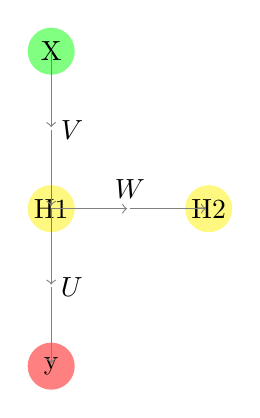
\begin{tikzpicture}[shorten >=1pt,->,draw=black!50, node distance=\layersep]
    		\tikzstyle{every pin edge}=[<-,shorten <=1pt]
    		\tikzstyle{neuron}=[circle,fill=black!25,minimum size=17pt,inner sep=0pt]
    		\tikzstyle{input neuron}=[neuron, fill=green!50];
    		\tikzstyle{hidden neuron}=[neuron, fill=yellow!50];
    		\tikzstyle{output neuron}=[neuron, fill=red!50];
    		\tikzstyle{annot} = [text width=4em, text centered]
    		
    		\node[input neuron] (I-1) at (0,0) {X};
    		\node[hidden neuron] (H-1) at (0,-2) {H1};
    		\draw (0,0) -- (0,-1) node(I-H11)[right] {$V$};
    		\draw (0,-1) -- (0,-2) node(I-H12)[right] {$$};
    		\node[output neuron] (O-1) at (0,-4) {y};
    		\draw (0,-2) -- (0,-3) node(H1-O1)[right] {$U$};
    		\draw (0,-3) -- (0,-4) node(H1-O2)[right] {$$};
    		\node[hidden neuron] (H-2) at (2,-2) {H2};
    		\draw (0,-2) -- (1,-2) node(H1-H21)[above] {$W$};
    		\draw (1,-2) -- (2,-2) node(H1-H22)[right] {$$};
    		
    	\end{tikzpicture}
    	\caption{Funcionamiento RNN}
    \end{figure}

    $V$ es el vector peso para la capa oculta, $U$ es el vector peso para la capa de salida y $W$ es el mismo vector peso para los diferentes instantes de tiempo. Teniendo en cuenta esto, se puede calcular la capa oculta y la salida teniendo en cuenta estas variables y la funci\'{o}n de activaci\'{o}n $\sigma$, para ello se usan las siguientes ecuaciones:
    
    \begin{align}
    	H_{t}=\sigma(UX_{t}+WH_{t-1})\\
    	y_{t}=Softmax(VH_{t})
    \end{align}

    RNN aplica el algoritmo \textit{backward propagation} para actualizar los pesos, sus fundamentos se exponen en el siguiente algoritmo LSTM.
  
    El algoritmo RNN a aplicar en el proyecto est\'{a} compuesto con una capa de RNN para el tratamiento de la informaci\'{o}n teniendo en cuenta los instantes de tiempo. Se Aplicar\'{a}n tres capas regularizadoras \textit{Dropout} no consecutivas con el objetivo de evitar el \textit{overfitting} y capas \textit{Dense} para redimensionar los datos, adem\'{a}s, se aplicar\'{a} el optimizador Adam. En conclusi\'{o}n, el algoritmo est\'{a} compuesto por $8$ capas divididos en: $1$ capa de salida, $1$ capa de RNN, $5$ capas de clasificaci\'{o}n y $1$ capa de salida. La arquitectura es la siguiente de forma secuencial:

\begin{enumerate}
	\item \textit{Input Layer}: Se introducen los datos originales con los pasos de tiempos.
	\item \textit{RNN layer}: Se aplica el proceso correspondiente al \textit{backpropagation} con pasos de tiempo.
	\item \textit{Dropout-1 layer}: Se aplica el regularizador \textit{Dropout} y comienza la clasificaci\'{o}n.
	\item \textit{Dense-1 layer}: Se comprimen los datos a 14 dimensiones.
	\item \textit{Dropout-2 layer}: Se aplica el nuevamente el regularizador.
	\item \textit{Dense-2 layer}: Se vuelve a aplicar la compresi\'{o}n de los datos.
	\item \textit{Dropout-3 layer}: Se vuelve a aplicar el regularizador.
	\item \textit{Dense-3 layer} o \textit{Output layer}: Se comprimen los datos a una dimensi\'{o}n terminando con la clasificaci\'{o}n de los datos.
\end{enumerate}

\begin{figure}[h!]
	\centering
	\begin{tikzpicture}[shorten >=1pt,->,draw=black!50, node distance=\layersep]
		\tikzstyle{every pin edge}=[<-,shorten <=1pt]
		\tikzstyle{neuron}=[circle,fill=black!25,minimum size=17pt,inner sep=0pt]
		\tikzstyle{input neuron}=[neuron, fill=green!50];
		\tikzstyle{fase1 neuron}=[neuron, fill=blue!50];
		\tikzstyle{fase2 neuron}=[neuron, fill=orange!50];
		\tikzstyle{output neuron}=[neuron, fill=red!50];
		\tikzstyle{annot} = [text width=4em, text centered]
		
		% Draw the input layer nodes
		\foreach \y in {1,...,7}{
			% This is the same as writing \foreach \name / \y in {1/1,2/2,3/3,4/4}
			\ifnum\y<4
			\node[input neuron, pin=left: \y] (I-\y) at (0,-\y) {};
			\fi
			\ifnum\y=4
			\node[input neuron, pin=left: \vdots] (I-\y) at (0,-\y) {};
			\fi
			\ifnum\y=5
			\node[input neuron, pin=left: 27] (I-\y) at (0,-\y) {};
			\fi
			\ifnum\y=6
			\node[input neuron, pin=left: 28] (I-\y) at (0,-\y) {};
			\fi
			\ifnum\y=7
			\node[input neuron, pin=left: 29] (I-\y) at (0,-\y) {};
			\fi
		}
		
		% Draw the RNN nodes
		\foreach \y in {1,...,7}
		\node[fase1 neuron, right of=I-4] (H1-\y) at (\layersep*0.5,-\y) {};
		
		% Draw the Dropout_1 nodes
		\foreach \y in {1,...,7}
		\node[fase2 neuron, right of=H1-4] (H2-\y) at (\layersep*2.3,-\y) {};
		
		% Draw the Dense_1 layer nodes
		\foreach \y in {1,...,5}
		\node[fase2 neuron, right of=H2-4] (H3-\y) at (\layersep*3.8,-\y cm) {};
		
		% Draw the Dropout_2 nodes
		\foreach \y in {1,...,5}
		\node[fase2 neuron, right of=H3-3] (H4-\y) at (\layersep*5.6,-\y cm) {};
		
		% Draw the Dense_2 nodes
		\foreach \y in {1,...,5}
		\node[fase2 neuron, right of=H4-3] (H5-\y) at (\layersep*7.5,-\y) {};
		
		% Draw the Dropout_3 layer nodes
		\foreach \y in {1,...,5}
		\node[fase2 neuron, right of=H5-3] (H6-\y) at (\layersep*9.1,-\y cm) {};
		
		% Draw the Dense_3 layer nodes
		\node[output neuron, right of=H6-3] (H7-1) at (\layersep*10.8,-1 cm) {};
		
		% Connect every node in the input layer with every node in the
		% RNN layer.
		\foreach \source in {1,...,7}
		\foreach \dest in {1,...,7}
		\path (I-\source) edge (H1-\dest);
		% Connect every node in the RNN layer with every node in the
		% Dropout_1 layer.
		\foreach \source in {1,...,7}
		\foreach \dest in {1,...,6}
		\path (H1-\source) edge (H2-\dest);
		% Connect every node in the Dropout_1 layer with every node in the
		% Dense_1 layer.
		\foreach \source in {1,...,6}
		\foreach \dest in {1,...,5}
		\path (H2-\source) edge (H3-\dest);
		% Connect every node in the Dense_1 layer with every node in the
		% Dropout_2 layer.
		\foreach \source in {1,...,5}
		\foreach \dest in {1,...,5}
		\path (H3-\source) edge (H4-\dest);
		% Connect every node in the Dropout_2 layer with every node in the
		% Dense_2 layer.
		\foreach \source in {1,...,5}
		\foreach \dest in {1,...,5}
		\path (H4-\source) edge (H5-\dest);
		% Connect every node in the Dense_2 layer with every node in the
		% Dropout_3 layer.
		\foreach \source in {1,...,5}
		\foreach \dest in {1,...,5}
		\path (H5-\source) edge (H6-\dest);
		% Connect every node in the Dropout_3 layer with every node in the
		% Dense_3 layer.
		\foreach \source in {1,...,5}
		\path (H6-\source) edge (H7-1);
		
		
		% Annotate the layers
		\node[annot,above of=H1-1, node distance=1cm] {RNN layer};
		\node[annot,above of=H2-1, node distance=1cm] {Dropout1 layer};
		\node[annot,above of=H3-1, node distance=1cm] {Dense1 layer};
		\node[annot,above of=H4-1, node distance=1cm] {Dropout2 layer};
		\node[annot,above of=H5-1, node distance=1cm] {Dense2 layer};
		\node[annot,above of=H6-1, node distance=1cm] {Dropout3 layer};
		\node[annot,above of=I-1] {Input layer};
		\node[annot,above of=H7-1] {Output layer};
	\end{tikzpicture}
\caption{Modelo RNN}
\end{figure}

\subsubsection{Long Short Term Memory (LSTM)}

    LSTM soluciona el problema de los gradientes que desaparecen y explotan de RNN al poseer una mayor memoria para almacenar los vectores de peso. La siguiente figura muestra la arquitectura del funcionamiento del algoritmo:
    
    \begin{figure}[h!]
    	\centering
    	\begin{tikzpicture}[shorten >=1pt,->,draw=black!50, node distance=\layersep]
    		\tikzstyle{every pin edge}=[<-,shorten <=1pt]
    		\tikzstyle{neuron}=[circle,fill=black!25,minimum size=17pt,inner sep=0pt]
    		\tikzstyle{input neuron}=[neuron, fill=green!100];
    		\tikzstyle{hidden state}=[neuron, fill=blue!50];
    		\tikzstyle{forget gate}=[neuron, fill=orange!50];
    		\tikzstyle{input gate}=[neuron, fill=cyan!50];
    		\tikzstyle{output gate}=[neuron, fill=gray!50];
    		\tikzstyle{cell state}=[neuron, fill=blue!100];
    		\tikzstyle{output neuron}=[neuron, fill=red!50];
    		\tikzstyle{annot} = [text width=4em, text centered]
    		
    		\node[input neuron] (I-1) at (0,-4) {X};
    		\node[hidden state] (H-1) at (\layersep*3,-4) {Hidden state};
    		\node[forget gate] (G-1) at (\layersep*6,-1) {Forget gate};
    		\node[input gate] (G-2) at (\layersep*9,-1) {Input gate};
    		\node[output gate] (G-3) at (\layersep*6,-7) {Output gate};
    		\node[cell state] (H-2) at (\layersep*6,-4) {Cell state};
    		\node[output neuron] (O-1) at (\layersep*9,-4) {y};
    		
    		\path (I-1) edge (H-1);
    		\path (H-1) edge (H-2);
    		\path (G-1) edge (H-2);
    		\path (G-2) edge (H-2);
    		\path (G-3) edge (H-2);
    		\path (H-2) edge (O-1);
    	\end{tikzpicture}
    \caption{Funcionamiento de LSTM}
    \end{figure}

  En la figura se denota $X$ como el conjunto de datos originales sin clasificar, este conjunto pasa al estado oculto (\textit{Hidden state}) que es similar a la capa RNN donde se alimenta de las entradas anteriores. Los datos pasan a tres puertas: \textit{Input gate}, \textit{Forget gate} y \textit{Output gate}, las cuales forman parte de la capa de memoria (\textit{Cell state}) que contiene los contextos de las entradas. \textit{Input gate}, decide si es necesario actualizar la memoria anterior de la red teniendo en cuenta a $X$. \textit{Forget gate}, decide si es necesario eliminar la memoria anterior de la red teniendo en cuenta a $X$. \textit{Output gate}, debe dar una salida y basada en la entrada actual, la salida de la capa anterior y la celda de memoria persistente.
  
  Teniendo en cuenta que $H^{'}$ es la salida del vector anterior con sus vectores de peso de la capa oculta $w^{'}$ y de la capa de entrada $u^{'}$. Estos vectores pesos se definen para cada una de las puertas, obteniendo $w_{1}^{'}$ y $u_{1}^{'}$ para \textit{forget gate}, $w_{2}^{'}$, $w_{3}^{'}$, $u_{2}^{'}$ y $u_{3}^{'}$ para \textit{input gate}, y $w_{4}^{'}$, $u_{4}^{'}$ para \textit{output gate}.
  
  \textbf{Forget gate}
  
  Esta puerta solo ajusta las dos entradas con pesos y se le aplica una funci\'{o}n de activaci\'{o}n para ajustar los valores de salida en $(0,1)$. Si el valor de entrada a esta puerta es $0$, al ser multiplicado con la celda de memoria, se podr\'{a}n eliminar los valores con \'{e}xito, por ello se llama la puerta de olvido. Se formaliza su ecuaci\'{o}n como:
  
  \begin{equation}
  	F=\sigma(u_{1}^{'}X+w_{1}^{'}H^{'})
  \end{equation}

\textbf{Input gate}

  Esta puerta lanza una salida a trav\'{e}s de la multiplicaci\'{o}n de dos funciones, el resultado de las funciones de activaci\'{o}n $\sigma$ y $\tan$. La responsabilidad de esta puerta es establecer el valor en el estado de la memoria, todos los valores se establecer\'{a}n, es por ello que se aplica $\sigma$ que establece el rango de los valores en $(0,1)$, luego se multiplican por $\tan$, que tiene un rango de valores entre $(-1,1)$. Teniendo en cuenta este resultado, se establecer\'{a}n en la memoria los valores que tienen valores que tienden a $1$ y los valores que tienden a $-1$ ser\'{a}n eliminados. Para establecer las ecuaciones se define $G$ como el estado candidato y a $I$ como el estado de entrada.
  
  \begin{align}
  	I=\sigma(u_{2}^{'}X+w_{2}^{'}H^{'})\\
  	G=\tan(u_{3}^{'}X+w_{3}^{'}H^{'})
  \end{align}

\textbf{Memory state}

  Una vez obtenidos los valores de \textit{forget gate} e \textit{input gate} se pueden calcular los valores de la memoria actual $C$ haciendo uso tambi\'{e}n de los valores anteriores de la memoria $C^{'}$.
  
  \begin{equation}
  	C=C^{'}F+IG
  \end{equation}

\textbf{Output gate}

  Esta puerta es b\'{a}sicamente la responsable de encontrar la salida final multiplicando las nuevas entradas y la memoria final. Se vuelve a multiplicar $C$ por $\tan$ para que el rango de salida sea $(-1,1)$ y sea mejor la eliminaci\'{o}n de valores si es necesario.
  
  \begin{align}
  	O=\tan(u_{4}^{'}X+w_{4}^{'}H^{'})\\
  	H^{'}=O\tan(C)\\
  	Output=vH^{'}
  \end{align}

  Hasta este momento se obtuvo la salida del \textit{forward propagation}, luego se aplica la t\'{e}cnica del \textit{backward propagation}. Las ecuaciones finales para obtener los nuevos pesos mediante la regla de la cadena para poder disminuir el error absoluto de las soluciones son:
  
  \begin{align}
  	E=\frac{(Output-Y)^2}{2}\\
  	w_{new}=w_{old}-\frac{\partial E}{\partial w}\\
  	v_{new}=v_{old}-\frac{\partial E}{\partial v}\\
  	u_{new}=u_{old}-\frac{\partial E}{\partial u}
  \end{align}

  Estas ecuaciones se aplican para los diferentes vectores de peso utilizados por las diferentes puertas de la memoria de valores.
  
  El algoritmo LSTM a aplicar en el proyecto est\'{a} compuesto con una capa LSTM para el tratamiento de la informaci\'{o}n teniendo en cuenta los instantes de tiempo. Se Aplicar\'{a}n tres capas regularizadoras \textit{Dropout} no consecutivas con el objetivo de evitar el \textit{overfitting} y capas \textit{Dense} para redimensionar los datos, adem\'{a}s, se aplicar\'{a} el optimizador Adam. En conclusi\'{o}n, el algoritmo est\'{a} compuesto por $8$ capas divididos en: $1$ capa de salida, $1$ capa de LSTM, $5$ capas de clasificaci\'{o}n y $1$ capa de salida. La arquitectura es la siguiente de forma secuencial:

\begin{enumerate}
	\item \textit{LSTM layer}: Se aplica el proceso correspondiente al \textit{backpropagation} con pasos de tiempo.
	\item \textit{Dropout-1 layer}: Se aplica el regularizador \textit{Dropout} y comienza la clasificaci\'{o}n.
	\item \textit{Dense-1 layer}: Se comprimen los datos a 14 dimensiones.
	\item \textit{Dropout-2 layer}: Se aplica el nuevamente el regularizador.
	\item \textit{Dense-2 layer}: Se vuelve a aplicar la compresi\'{o}n de los datos.
	\item \textit{Dropout-3 layer}: Se vuelve a aplicar el regularizador.
	\item \textit{Dense-3 layer} o \textit{Output layer}: Se comprimen los datos a una dimensi\'{o}n terminando con la clasificaci\'{o}n de los datos.
\end{enumerate}

\begin{figure}[h!]
	\centering
	\begin{tikzpicture}[shorten >=1pt,->,draw=black!50, node distance=\layersep]
		\tikzstyle{every pin edge}=[<-,shorten <=1pt]
		\tikzstyle{neuron}=[circle,fill=black!25,minimum size=17pt,inner sep=0pt]
		\tikzstyle{input neuron}=[neuron, fill=green!50];
		\tikzstyle{fase1 neuron}=[neuron, fill=blue!50];
		\tikzstyle{fase2 neuron}=[neuron, fill=orange!50];
		\tikzstyle{output neuron}=[neuron, fill=red!50];
		\tikzstyle{annot} = [text width=4em, text centered]
		
		% Draw the input layer nodes
		\foreach \y in {1,...,7}{
			% This is the same as writing \foreach \name / \y in {1/1,2/2,3/3,4/4}
			\ifnum\y<4
			\node[input neuron, pin=left: \y] (I-\y) at (0,-\y) {};
			\fi
			\ifnum\y=4
			\node[input neuron, pin=left: \vdots] (I-\y) at (0,-\y) {};
			\fi
			\ifnum\y=5
			\node[input neuron, pin=left: 27] (I-\y) at (0,-\y) {};
			\fi
			\ifnum\y=6
			\node[input neuron, pin=left: 28] (I-\y) at (0,-\y) {};
			\fi
			\ifnum\y=7
			\node[input neuron, pin=left: 29] (I-\y) at (0,-\y) {};
			\fi
		}
		
		% Draw the LSTM nodes
		\foreach \y in {1,...,7}
		\node[fase1 neuron, right of=I-4] (H1-\y) at (\layersep*0.5,-\y) {};
		
		% Draw the Dropout_1 nodes
		\foreach \y in {1,...,7}
		\node[fase2 neuron, right of=H1-4] (H2-\y) at (\layersep*2.3,-\y) {};
		
		% Draw the Dense_1 layer nodes
		\foreach \y in {1,...,5}
		\node[fase2 neuron, right of=H2-4] (H3-\y) at (\layersep*3.8,-\y cm) {};
		
		% Draw the Dropout_2 nodes
		\foreach \y in {1,...,5}
		\node[fase2 neuron, right of=H3-3] (H4-\y) at (\layersep*5.6,-\y cm) {};
		
		% Draw the Dense_2 nodes
		\foreach \y in {1,...,5}
		\node[fase2 neuron, right of=H4-3] (H5-\y) at (\layersep*7.5,-\y) {};
		
		% Draw the Dropout_3 layer nodes
		\foreach \y in {1,...,5}
		\node[fase2 neuron, right of=H5-3] (H6-\y) at (\layersep*9.1,-\y cm) {};
		
		% Draw the Dense_3 layer nodes
		\node[output neuron, right of=H6-3] (H7-1) at (\layersep*10.8,-1 cm) {};
		
		% Connect every node in the input layer with every node in the
		% LSTM layer.
		\foreach \source in {1,...,7}
		\foreach \dest in {1,...,7}
		\path (I-\source) edge (H1-\dest);
		% Connect every node in the LSTM layer with every node in the
		% Dropout_1 layer.
		\foreach \source in {1,...,7}
		\foreach \dest in {1,...,6}
		\path (H1-\source) edge (H2-\dest);
		% Connect every node in the Dropout_1 layer with every node in the
		% Dense_1 layer.
		\foreach \source in {1,...,6}
		\foreach \dest in {1,...,5}
		\path (H2-\source) edge (H3-\dest);
		% Connect every node in the Dense_1 layer with every node in the
		% Dropout_2 layer.
		\foreach \source in {1,...,5}
		\foreach \dest in {1,...,5}
		\path (H3-\source) edge (H4-\dest);
		% Connect every node in the Dropout_2 layer with every node in the
		% Dense_2 layer.
		\foreach \source in {1,...,5}
		\foreach \dest in {1,...,5}
		\path (H4-\source) edge (H5-\dest);
		% Connect every node in the Dense_2 layer with every node in the
		% Dropout_3 layer.
		\foreach \source in {1,...,5}
		\foreach \dest in {1,...,5}
		\path (H5-\source) edge (H6-\dest);
		% Connect every node in the Dropout_3 layer with every node in the
		% Dense_3 layer.
		\foreach \source in {1,...,5}
		\path (H6-\source) edge (H7-1);
		
		
		% Annotate the layers
		\node[annot,above of=H1-1, node distance=1cm] {LSTM layer};
		\node[annot,above of=H2-1, node distance=1cm] {Dropout1 layer};
		\node[annot,above of=H3-1, node distance=1cm] {Dense1 layer};
		\node[annot,above of=H4-1, node distance=1cm] {Dropout2 layer};
		\node[annot,above of=H5-1, node distance=1cm] {Dense2 layer};
		\node[annot,above of=H6-1, node distance=1cm] {Dropout3 layer};
		\node[annot,above of=I-1] {Input layer};
		\node[annot,above of=H7-1] {Output layer};
	\end{tikzpicture}
	\caption{Modelo LSTM}
\end{figure}

  Ya concluida la presentaci\'{o}n y fundamentaci\'{o}n del funcionamiento y estructura de los algoritmos de DL a utilizar en el proyecto, es posible proceder a la evaluaci\'{o}n de los algoritmos. La evaluaci\'{o}n y aplicaci\'{o}n del conocimiento forman los pasos finales de la metodolog\'{i}a aplicada para el desarrollo del proyecto. Para la evaluaci\'{o}n de los algoritmos se realizar\'{a}n $7$ experimentos que ser\'{a}n detallados y representados sus resultados en el siguiente cap\'{i}tulo, y finalizando el mismo la aplicaci\'{o}n del conocimiento adquirido.